%{{第七十四回}}{第七十四回}}
\chapter{惑奸谗抄检大观园\\矢孤介杜绝宁国府}\label{part0078_split_000.htmlux5cux23calibre_pb_0}
{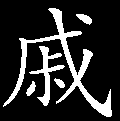
\includegraphics[width=3mm]{../Images/00005}\kaishu 司棋一事,在七十一回叙明,暗用山石伏线,七十三回用绣春囊在山石一逗便住,至此回可直叙去,又用无数曲折渐渐逼来,及至司棋,忽然顿住,结到入画。文气如黄河出昆仑,横流数万里,九曲至龙门,又有孟门、吕梁峡束,不得入海。是何等奇险怪特文字,令我拜服!}

话说平儿听迎春说了正自好笑,忽见宝玉也来了。原来管厨房柳家媳妇之妹,也因放头开赌得了不是。这园中有素与柳家不睦的,{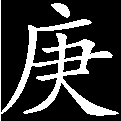
\includegraphics[width=3mm]{../Images/00004}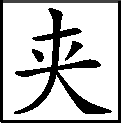
\includegraphics[width=3mm]{../Images/00012}\footnotesize \kaishu 前文已卯之伏线。}便又告出柳家来,说他和他妹子是伙计,虽然他妹子出名,其实赚了钱两个人平分。因此凤姐要治柳家之罪。那柳家的因得此信,便慌了手脚,因思素与怡红院人最为深厚,故走来悄悄地央求晴雯、金星玻璃等人。金星玻璃告诉了宝玉。宝玉因思内中迎春之乳母也现有此罪,不若来约同迎春讨情,比自己独去单为柳家说情又更妥当,故此前来。忽见许多人在此,见他来时,都问:``你的病可好了?跑来作什么?''宝玉不便说出讨情一事,只说:``来看二姐姐。''当下众人也不在意,且说些闲话。平儿便出去办累丝金凤一事。那王住儿媳妇紧跟在后,口内百般央求,只说:``姑娘好歹口内超生,我横竖去赎了来。''平儿笑道:``你迟也赎,早也赎,既有今日,何必当初。你的意思得过去就过去了。既是这样,我也不好意思告人,趁早去赎了来交与我送去,我一字不提。''王住儿媳妇听说,方放下心来,就拜谢,又说:``姑娘自去贵干,我赶晚拿了来,先回了姑娘,再送去,如何?''平儿道:``赶晚不来,可别怨我。''说毕,二人方分路各自散了。

平儿到房,凤姐问他:``三姑娘叫你作什么?''平儿笑道:``三姑娘怕奶奶生气,叫我劝着奶奶些,问奶奶这两天可吃些什么。''凤姐笑道:``倒是他还记挂着我。刚才又出来了一件事:有人来告柳二媳妇和他妹子通同开局,凡妹子所为,都是他作主。我想,你素日肯劝我`多一事不如省一事',就可闲一时心,自己保养保养也是好的。我因听不进去,果然应了些,先把太太得罪了,而且自己反赚了一场病。如今我也看破了,随他们闹去罢,横竖还有许多人呢。我白操一会子心,倒惹的万人咒骂。我且养病要紧,便是好了,我也作个好好先生,得乐且乐,得笑且笑,一概是非都凭他们去罢。{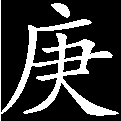
\includegraphics[width=3mm]{../Images/00004}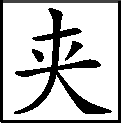
\includegraphics[width=3mm]{../Images/00012}\footnotesize \kaishu 历来世人到此作此想,但悔不及矣。可伤可叹。}所以我只答应着知道了,白不在我心上。''平儿笑道:``奶奶果然如此,便是我们的造化。''

一语未了,只见贾琏进来,拍手叹气道:``好好的又生事。前儿我和鸳鸯借当,那边太太怎么知道了。才刚太太叫过我去,叫我不管那里先迁挪二百银子,做八月十五日节间使用。我回没处迁挪。太太就说:`你没有钱就有地方迁挪,我白和你商量,你就搪塞我,你就说没地方。前儿一千银子的当是那里的?连老太太的东西你都有神通弄出来,这会子二百银子,你就这样。幸亏我没和别人说去。'我想太太分明不短,何苦来要寻事奈何人。''凤姐儿道:``那日并没一个外人,谁走了这个消息?''平儿听了,也细想那日有谁在此,想了半日,笑道:``是了。那日说话时没一个外人,但晚上送东西来的时节,老太太那边傻大姐的娘也可巧来送浆洗衣服。他在下房里坐了一会子,见一大箱子东西,自然要问,必是小丫头们不知道,说了出来,也未可知。''{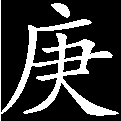
\includegraphics[width=3mm]{../Images/00004}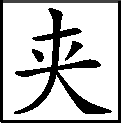
\includegraphics[width=3mm]{../Images/00012}\footnotesize \kaishu 奇奇怪怪,从何处转至素日{(成)}{[}来{]},真如常山之蛇。}因此便唤了几个小丫头来问,那日谁告诉呆大姐的娘。众小丫头慌了,都跪下赌咒发誓,说:``自来也不敢多说一句话。有人凡问什么,都答应不知道。这事如何敢多说。''凤姐详情说:``他们必不敢,倒别委屈了他们。如今且把这事靠后,且把太太打发了去要紧。宁可咱们短些,又别讨没意思。''因叫平儿:``把我的金项圈拿来,且去暂押二百银子来送去完事。''贾琏道:``越性多押二百,咱们也要使呢。''凤姐道:``很不必,我没处使钱。这一去还不知指那一项赎呢。''平儿拿去,吩咐一个人唤了旺儿媳妇来领去,不一时拿了银子来。贾琏亲自送去,不在话下。

这里凤姐和平儿猜疑,终是谁人走的风声,竟拟不出人来。凤姐儿又道:``知道这事还是小事,怕的是小人趁便又造非言,生出别的事来。当紧那边正和鸳鸯结下仇了,如今听得他私自借给琏二爷东西,那起小人眼馋肚饱,连没缝儿的鸡蛋还要下蛆呢,如今有了这个因由,恐怕又造出些没天理的话来也定不得。在你琏二爷还无妨,只是鸳鸯正经女儿,带累了他受屈,岂不是咱们的过失。''平儿笑道:``这也无妨。鸳鸯借东西看的是奶奶,并不为的是二爷。一则鸳鸯虽应名是他私情,其实他是回过老太太的。老太太因怕孙男弟女多,这个也借,那个也要,到跟前撒个娇儿,和谁要去,\elegantpar{因此只装不知道。}{是也。}{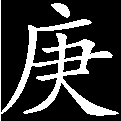
\includegraphics[width=3mm]{../Images/00004}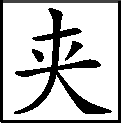
\includegraphics[width=3mm]{../Images/00012}\footnotesize \kaishu 奇文神文!岂世人{(余相)}{[}意想{]}得出者?前文云``一箱子'',若是私拿出,贾母其睡梦中之人矣。盖此等事作者曾经,批者曾经,实系一写往事,非特造出,故弄新笔,究竟不记不神也。◇鸳鸯借物一回于此便结了。}纵闹了出来,究竟那也无碍。''凤姐儿道:``理固如此。只是你我是知道的,那不知道的,焉得不生疑呢。''

一语未了,人报:``太太来了。''凤姐听了诧异,不知为何事亲来,与平儿等忙迎出来。只见王夫人气色更变,{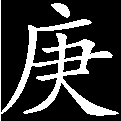
\includegraphics[width=3mm]{../Images/00004}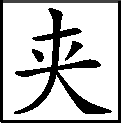
\includegraphics[width=3mm]{../Images/00012}\footnotesize \kaishu 奇。}只带一个贴己的小丫头走来,一语不发,走至里间坐下。凤姐忙奉茶,因陪笑问道:``太太今日高兴,到这里逛逛。''王夫人喝命:``平儿出去!''平儿见了这般,着慌不知怎么样了,忙应了一声,带着众小丫头一齐出去,在房门外站住,越性将房门掩了,自己坐在台矶上,所有的人,一个不许进去。凤姐也着了慌,不知有何等事。只见王夫人含着泪,从袖内掷出一个香袋子来,说:``你瞧。''凤姐忙拾起一看,见是十锦春意香袋,也吓了一跳,忙问:``太太从那里得来?''王夫人见问,越发泪如雨下,颤声说道:``我从那里得来!我天天坐在井里,拿你当个细心人,所以我才偷个空儿。谁知你也和我一样。这样的东西大天白日明摆在园里山石上,被老太太的丫头拾着,不亏你婆婆遇见,早已送到老太太跟前去了。我且问你,这个东西如何遗在那里来?''{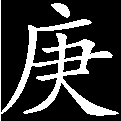
\includegraphics[width=3mm]{../Images/00004}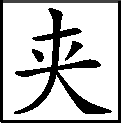
\includegraphics[width=3mm]{../Images/00012}\footnotesize \kaishu 奇问。}凤姐听得,也更了颜色,忙问:``太太怎知是我的?''{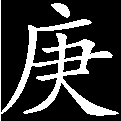
\includegraphics[width=3mm]{../Images/00004}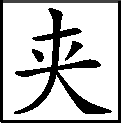
\includegraphics[width=3mm]{../Images/00012}\footnotesize \kaishu 问的是。}王夫人又哭又叹说道:``你反问我!你想,一家子除了你们小夫小妻,馀者老婆子们,要这个何用?再女孩子们是从那里得来?自然是那琏儿不长进下流种子那里弄来。你们又和气。当作一件顽意儿,年轻人儿女闺房私意是有的,你还和我赖!幸而园内上下人还不解事,尚未拣得。倘或丫头们拣着,你姊妹看见,这还了得。不然有那小丫头们拣着,出去说是园内拣着的,外人知道,这性命脸面要也不要?''

凤姐听说,又急又愧,登时紫涨了面皮,便依炕沿双膝跪下,也含泪诉道:``太太说的固然有理,我也不敢辩我并无这样的东西。但其中还要求太太细详其理:那香袋是外头雇工仿着内工绣的,带这穗子一概是市卖货。我便年轻不尊重些,也不要这劳什子,自然都是好的,此其一。二者这东西也不是常带着的,我纵有,也只好在家里,焉肯带在身上各处去?况且又在园里去,个个姊妹我们都肯拉拉扯扯,倘或露出来,不但在姊妹前,就是奴才看见,我有什么意思?我虽年轻不尊重,亦不能糊涂至此。三则论主子内我是年轻媳妇,算起奴才来,比我更年轻的又不止一个人了。况且他们也常进园,晚间各人家去,焉知不是他们身上的?四则除我常在园里之外,还有那边太太常带过几个小姨娘来,如嫣红翠云等人,皆系年轻侍妾,他们更该有这个了。还有那边珍大嫂子,他不算甚老外,他也常带过配凤等人来,焉知又不是他们的?五则园内丫头太多,保的住个个都是正经的不成?也有年纪大些的知道了人事,或者一时半刻人查问不到偷着出去,或借着因由同二门上小幺儿们打牙犯嘴,外头得了来的,也未可知。如今不但我没此事,就连平儿我也可以下保的。太太请细想。''

王夫人听了这一席话大近情理,因叹道:``你起来。我也知道你是大家小姐出身,焉得轻薄至此,不过我气急了,拿了话激你。但如今却怎么处?你婆婆才打发人封了这个给我瞧,说是前日从傻大姐手里得的,把我气了个死。''凤姐道:``太太快别生气。若被众人觉察了,保不定老太太不知道。且平心静气暗暗访察,才得确实,纵然访不着,外人也不能知道。这叫作`\elegantpar{胳膊折在袖内}{第三回}'。如今惟有趁着赌钱的因由革了许多的人这空儿,把周瑞媳妇旺儿媳妇等四五个贴近不能走话的人安插在园里,以查赌为由。再如今他们的丫头也太多了,保不住人大心大,生事作耗,等闹出事来,反悔之不及。如今若无故裁革,不但姑娘们委屈烦恼,就连太太和我也过不去。不如趁此机会,以后凡年纪大些的,或有些咬牙难缠的,拿个错儿撵出去配了人。一则保得住没有别的事,二则也可省些用度。太太想我这话如何?''王夫人叹道:``你说的何尝不是,但从公细想,你这几个姊妹也甚可怜了。{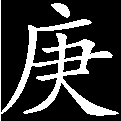
\includegraphics[width=3mm]{../Images/00004}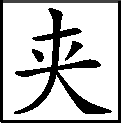
\includegraphics[width=3mm]{../Images/00012}\footnotesize \kaishu 犹云``可怜'',妙文!在别人视之,今古无比矣;若在荣府论,实不能比先矣。}也不用远比,只说如今你林妹妹的母亲,未出阁时,是何等的娇生惯养,是何等的金尊玉贵,那才像个千金小姐的体统。如今这几个姊妹,不过比人家的丫头略强些罢了。{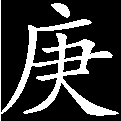
\includegraphics[width=3mm]{../Images/00004}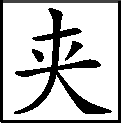
\includegraphics[width=3mm]{../Images/00012}\footnotesize \kaishu 所谓``\elegantpar{观于海者难为水}{观于海者难为水}'',俗子谓王夫人不知足,是不可矣;又谓作太过,真蟪蛄、学鸠之见也。}\href{../Text/part0078_split_000.html\#lnkback_1_a}{\textsuperscript{①}}通共每人只有两三个丫头像个人样,馀者纵有四五个小丫头子,竟是庙里的小鬼。如今还要裁革了去,不但于我心不忍,只怕老太太未必就依。虽然艰难,难不至此。我虽没受过大荣华富贵,比你们是强的。如今我宁可省些,别委曲了他们。以后要省俭先从我来倒使得。如今且叫人传了周瑞家的等人进来,就吩咐他们快快暗地访拿这事要紧。''凤姐听了,即唤平儿进来吩咐出去。

一时,周瑞家的与吴兴家的、郑华家的、来旺家的、来喜家的现在五家陪房进来,馀者皆在南方各有执事。{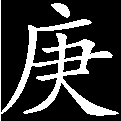
\includegraphics[width=3mm]{../Images/00004}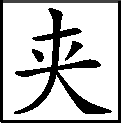
\includegraphics[width=3mm]{../Images/00012}\footnotesize \kaishu 又伏一笔。}王夫人正嫌人少不能勘察,忽见邢夫人的陪房王善保家的走来,方才正是他送香囊来的。王夫人向来看视邢夫人之得力心腹人等原无二意,{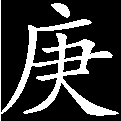
\includegraphics[width=3mm]{../Images/00004}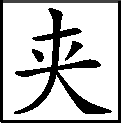
\includegraphics[width=3mm]{../Images/00012}\footnotesize \kaishu 大书。看下人犹如此,可知待邢夫人矣。}今见他来打听此事,十分关切,{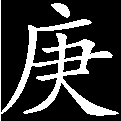
\includegraphics[width=3mm]{../Images/00004}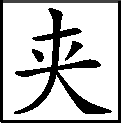
\includegraphics[width=3mm]{../Images/00012}\footnotesize \kaishu 小人外是内非,{(委)}{[}悉{]}皆如此。}便向他说:``你去回了太太,也进园内照管照管,不比别人又强些。''

这王善保家正因素日进园去那些丫鬟们不大趋奉他,他心里大不自在,要寻他们的故事又寻不着,恰好生出这事来,以为得了把柄。又听王夫人委托,正撞在心坎上,说:``这个容易。不是奴才多话,论理这事该早严紧的。太太也不大往园里去,这些女孩子们一个个倒像受了封诰似的,他们就成了千金小姐了。闹下天来,谁敢哼一声儿。不然,就调唆姑娘的丫头们,说欺负了姑娘们了,谁还耽得起。''王夫人道:``这也有的常情,跟姑娘的丫头原比别的娇贵些。你们该劝他们。连主子们的姑娘不教导尚且不堪,何况他们。''王善保家的道:``别的都还罢了。太太不知道,一个宝玉屋里的晴雯,那丫头仗着他生的模样儿比别人标致些,又生了一张巧嘴,\elegantpar{天天打扮的像个西施的样子}{这边讲晴雯样貌},在人跟前能说惯道,掐尖要强。一句话不投机,他就立起两个骚眼睛来骂人,妖妖趫趫,大不成个体统。''{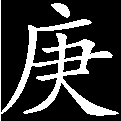
\includegraphics[width=3mm]{../Images/00004}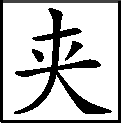
\includegraphics[width=3mm]{../Images/00012}\footnotesize \kaishu 活画出晴雯来。可知已前知晴雯必应遭妒者,可怜可伤,竟死矣。}

王夫人听了这话,猛然触动往事,便问凤姐道:``上次我们跟了老太太进园逛去,有一个水蛇腰,{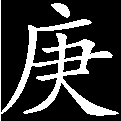
\includegraphics[width=3mm]{../Images/00004}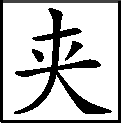
\includegraphics[width=3mm]{../Images/00012}\footnotesize \kaishu 妙妙,好腰!}削肩膀,{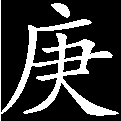
\includegraphics[width=3mm]{../Images/00004}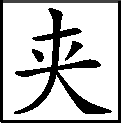
\includegraphics[width=3mm]{../Images/00012}\footnotesize \kaishu 妙妙,好肩!◇俗云:``水蛇腰则游曲小也。''又云:``美人无肩。''又曰:``肩若削成。''}\href{../Text/part0078_split_000.html\#lnkback_2_a}{\textsuperscript{②}}{皆是美之形也。凡写美人偏用俗笔反笔,与他书不同也。}眉眼又有些像你林妹妹的,{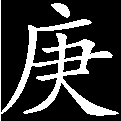
\includegraphics[width=3mm]{../Images/00004}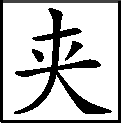
\includegraphics[width=3mm]{../Images/00012}\footnotesize \kaishu 更好,形容尽矣。}正在那里骂小丫头。我的心里很看不上那狂样子,因同老太太走,我不曾说得。后来要问是谁,又偏忘了。今日对了坎儿,这丫头想必就是他了。''凤姐道:``若论这些丫头们,共总比起来,都没晴雯生得好。论举止言语,他原有些轻薄。方才太太说的倒很像他,我也忘了那日的事,不敢乱说。''王善保家的便道:``不用这样,此刻不难叫了他来太太瞧瞧。''王夫人道:``宝玉房里常见我的只有袭人麝月,这两个笨笨的倒好。若有这个,他自不敢来见我的。我一生最嫌这样人,况且又出来这个事。\elegantpar{好好的宝玉,倘或叫这蹄子勾引坏了}{自己的儿子就好好的,别人的女儿就骚蹄子,金钏儿也死在最仁厚的手里}'因叫自己的丫头来,吩咐他:``到园里去,只说我说有话问他们,留下袭人麝月伏侍宝玉不必来,有一个晴雯最伶俐,叫他即刻快来。你不许和他说什么。''

小丫头子答应了,走入怡红院,正值晴雯身上不自在,睡中觉才起来,正发闷,听如此说,只得随了他来。素日这些丫鬟皆知王夫人最嫌趫妆艳饰语薄言轻者,故晴雯不敢出头。今因连日不自在,{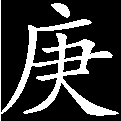
\includegraphics[width=3mm]{../Images/00004}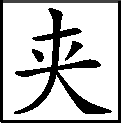
\includegraphics[width=3mm]{../Images/00012}\footnotesize \kaishu {(音)}{[}摹{]}神之至!}\href{../Text/part0078_split_000.html\#lnkback_3_a}{\textsuperscript{③}}{所谓``魂早离舍''矣,将死之兆也。◇若俗笔必云十分妆饰,今云不自在,想无挂心之态,更不入王夫人之眼也。}并没十分妆饰,自为无碍。{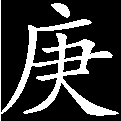
\includegraphics[width=3mm]{../Images/00004}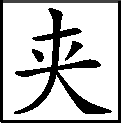
\includegraphics[width=3mm]{../Images/00012}\footnotesize \kaishu 好!可知天生美人原不在妆饰,使人一见不觉心惊目骇。可恨世之涂脂抹粉,真同鬼魅而不见觉。}及到了凤姐房中,王夫人一见他钗軃鬓松,衫垂带褪,有春睡捧心之遗风,而且形容面貌恰是上月的那人,不觉勾起方才的火来。

王夫人原是天真烂漫之人,喜怒出于心臆,不比那些饰词掩意之人,今既真怒攻心,又勾起往事,便冷笑道:``好个美人!真像个病西施了。你天天作这轻狂样儿给谁看?你干的事,打量我不知道呢!我且放着你,自然明儿揭你的皮!宝玉今日可好些?''晴雯一听如此说,心内大异,便知有人暗算了他。虽然着恼,只不敢作声。他本是个聪明过顶的人,{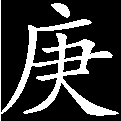
\includegraphics[width=3mm]{../Images/00004}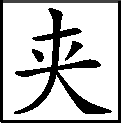
\includegraphics[width=3mm]{../Images/00012}\footnotesize \kaishu 深罪聪明,到底不错一笔。}见问宝玉可好些,他便不肯以实话对,只说:``我不大到宝玉房里去,又不常和宝玉在一处,好歹我不能知,这只问袭人麝月两个。''王夫人道:``这就该打嘴!你难道是死人,要你们作什么!''晴雯道:``我原是跟老太太的人。因老太太说园里空大人少,宝玉害怕,所以拨了我去外间屋里上夜,不过填屋子。我原回过我笨,不能伏侍。老太太骂了我,说:`又不叫你管他的事,要伶俐的作什么。'我听了这话才去的。不过十天半个月之内,宝玉闷了大家顽一会子就散了。至于宝玉饮食起坐,上一层有老奶奶老妈妈们,下一层又有袭人、麝月、秋纹几个人。我闲着还要作老太太屋里的针线,所以宝玉的事竟不曾留心。太太既怪,从此后我留心就是了。''王夫人信以为实了,忙说:``阿弥陀佛!你不近宝玉是我的造化,竟不劳你费心。既是老太太给宝玉的,我明儿回了老太太,再撵你。''因向王善保家的道:``你们进去,好生防他几日,不许他在宝玉房里睡觉。等我回过老太太,再处治他。''喝声``去!站在这里,我看不上这浪样儿!谁许你这样花红柳绿的妆扮!''晴雯只得出来,这气非同小可,一出门便拿手帕子握着脸,一头走,一头哭,直哭到园门内去。

这里王夫人向凤姐等自怨道:``这几年我越发精神短了,照顾不到。这样妖精似的东西竟没看见。只怕这样的还有,明日倒得查查。''凤姐见王夫人盛怒之际,又因王善保家的是邢夫人的耳目,常调唆着邢夫人生事,纵有千百样言词,此刻也不敢说,只低头答应着。王善保家的道:``太太请养息身体要紧,这些小事只交与奴才。如今要查这个主儿也极容易,等到晚上园门关了的时节,内外不通风,我们竟给他们个猛不防,带着人到各处丫头们房里搜寻。想来谁有这个,断不单只有这个,自然还有别的东西。那时翻出别的来,自然这个也是他的。''王夫人道:``这话倒是。若不如此,断不能清的清白的白。''因问凤姐如何。凤姐只得答应说:``太太说的是,就行罢了。''王夫人道:``这主意很是,不然一年也查不出来。''于是大家商议已定。

至晚饭后,待贾母安寝了,宝钗等入园时,王善保家的便请了凤姐一并入园,喝命将角门皆上锁,便从上夜的婆子处抄检起,不过抄检出些多馀攒下蜡烛灯油等物。{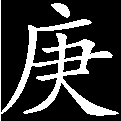
\includegraphics[width=3mm]{../Images/00004}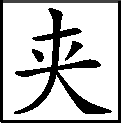
\includegraphics[width=3mm]{../Images/00012}\footnotesize \kaishu 毕真。}王善保家的道:``这也是赃,不许动,等明儿回过太太再动。''于是先就到怡红院中,喝命关门。当下宝玉正因晴雯不自在,忽见这一干人来,不知为何直扑了丫头们的房门去,因迎出凤姐来,问是何故。凤姐道:``丢了一件要紧的东西,因大家混赖,恐怕有丫头们偷了,所以大家都查一查去疑。''一面说,一面坐下吃茶。王善保家的等搜了一回,又细问这几个箱子是谁的,都叫本人来亲自打开。袭人因见晴雯这样,知道必有异事,又见这番抄检,只得自己先出来打开了箱子并匣子,任其搜检一番,不过是平常动用之物。随放下又搜别人的,挨次都一一搜过。到了晴雯的箱子,因问:``是谁的,怎不开了让搜?''袭人等方欲代晴雯开时,只见晴雯挽着头发闯进来,``豁''一声将箱子掀开,两手捉着,底子朝天往地下尽情一倒,将所有之物尽都倒出。王善保家的也觉没趣,\href{../Text/part0078_split_000.html\#lnkback_4_a}{\textsuperscript{④}}看了一看,也无甚私弊之物。回了凤姐,要往别处去。凤姐儿道:``你们可细细的查,若这一番查不出来,难回话的。''众人都道:``都细翻看了,没什么差错东西。虽有几样男人物件,都是小孩子的东西,想是宝玉的旧物件,没甚关系的。''凤姐听了,笑道:``既如此咱们就走,再瞧别处去。''

说着,一径出来,因向王善保家的道:``我有一句话,不知是不是。要抄检只抄检咱们家的人,薛大姑娘屋里,断乎检抄不得的。''王善保家的笑道:``这个自然。岂有抄起亲戚家来。''凤姐点头道:``我也这样说呢。''{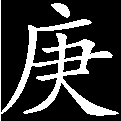
\includegraphics[width=3mm]{../Images/00004}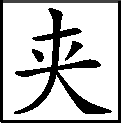
\includegraphics[width=3mm]{../Images/00012}\footnotesize \kaishu 写阿凤心灰意懒,且避祸从时,迥又是一个人矣。}一头说,一头到了潇湘馆内。黛玉已睡了,忽报这些人来,也不知为甚事。才要起来,只见凤姐已走进来,忙按住他不许起来,只说:``睡罢,我们就走。''这边且说些闲话。那个王善保家的带了众人到丫鬟房中,也一一开箱倒笼抄检了一番。因从紫鹃房中抄出两副宝玉常换下来的寄名符儿,一副束带上的披带,两个荷包并扇套,套内有扇子。打开看时皆是宝玉往年往日手内曾拿过的。王善保家的自为得了意,遂忙请凤姐过来验视,又说:``这些东西从那里来的?''凤姐笑道:``宝玉和他们从小儿在一处混了几年,这自然是宝玉的旧东西。这也不算什么罕事,撂下再往别处去是正经。''紫鹃笑道:``直到如今,我们两下里的东西也算不清。要问这一个,连我也忘了是那年月日有的了。''王善保家的听凤姐如此说,也只得罢了。{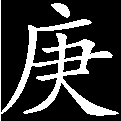
\includegraphics[width=3mm]{../Images/00004}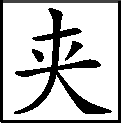
\includegraphics[width=3mm]{../Images/00012}\footnotesize \kaishu 一处一样。}

又到探春院内,谁知早有人报与探春了。{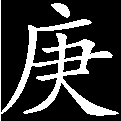
\includegraphics[width=3mm]{../Images/00004}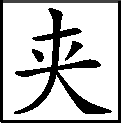
\includegraphics[width=3mm]{../Images/00012}\footnotesize \kaishu 不板。}探春也就猜着必有原故,所以引出这等丑态来,{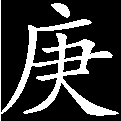
\includegraphics[width=3mm]{../Images/00004}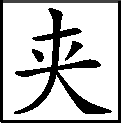
\includegraphics[width=3mm]{../Images/00012}\footnotesize \kaishu 实注一笔。}遂命众丫鬟秉烛开门而待。一时,众人来了。探春故问何事。凤姐笑道:``因丢了一件东西,连日访察不出人来,恐怕旁人赖这些女孩子们,所以越性大家搜一搜,使人去疑,倒是洗净他们的好法子。''探春冷笑道:``我们的丫头自然都是些贼,我就是头一个窝主。既如此,先来搜我的箱柜,他们所有偷了来的都交给我藏着呢。''说着便命丫头们把箱柜一齐打开,将镜奁、妆盒、衾袱、衣包若大若小之物一齐打开,请凤姐去抄阅。凤姐陪笑道:``我不过是奉太太的命来,妹妹别错怪我。何必生气。''因命丫鬟们快快关上。

平儿丰儿等忙着替待书等关的关,收的收。探春道:``我的东西倒许你们搜阅,要想搜我的丫头,这却不能。我原比众人歹毒,凡丫头所有的东西我都知道,都在我这里间收着,一针一线他们也没的收藏,要搜所以只来搜我。你们不依,只管去回太太,只说我违背了太太,该怎么处治,我去自领。你们别忙,自然连你们抄的日子有呢!你们今日早起不曾议论甄家,\elegantpar{自己家里好好的抄家}{甄家也抄过自己家},果然今日真抄了。{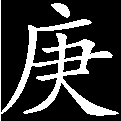
\includegraphics[width=3mm]{../Images/00004}\includegraphics[width=3mm]{../Images/00012}\footnotesize \kaishu 奇极!此日甄家事。}咱们也渐渐的来了。可知这样大族人家,若从外头杀来,一时是杀不死的,这是古人曾说的`百足之虫,死而不僵',必须先从家里自杀自灭起来,才能一败涂地!''说着,不觉流下泪来。

凤姐只看着众媳妇们。周瑞家的便道:``既是女孩子的东西全在这里,奶奶且请到别处去罢,也让姑娘好安寝。''凤姐便起身告辞。探春道:``可细细的搜明白了?若明日再来,我就不依了。''凤姐笑道:``既然丫头们的东西都在这里,就不必搜了。''探春冷笑道:``你果然倒乖。连我的包袱都打开了,还说没翻。明日敢说我护着丫头们,不许你们翻了。你趁早说明,若还要翻,不妨再翻一遍。''凤姐知道探春素日与众不同的,只得陪笑道:``我已经连你的东西都搜查明白了。''探春又问众人:``你们也都搜明白了不曾?''周瑞家的等都陪笑说:``都翻明白了。''

那王善保家的本是个心内没成算的人,素日虽闻探春的名,那是为众人没眼力没胆量罢了,那里一个姑娘家就这样起来,况且又是庶出,他敢怎么。他自恃是邢夫人陪房,连王夫人尚另眼相看,何况别个。今见探春如此,他只当是探春认真单恼凤姐,与他们无干。他便要趁势作脸献好,因越众向前拉起探春的衣襟,故意一掀,嘻嘻笑道:``连姑娘身上我都翻了,果然没有什么。''凤姐见他这样,忙说:``妈妈走罢,别疯疯颠颠的。''一语未了,只听``拍''的一声,王家的脸上早着了探春一掌。探春登时大怒,指着王家的问道:``你是什么东西,敢来拉扯我的衣裳!我不过看着太太的面上,你又有年纪,叫你一声妈妈,你就狗仗人势,天天作耗,专管生事。如今越性了不得了。你打量我是同你们姑娘那样好性儿,由着你们欺负他,就错了主意!你搜检东西我不恼,你不该拿我取笑。''说着,便亲自解衣卸裙,拉着凤姐儿细细的翻。又说:``省得叫奴才来翻我身上。''凤姐平儿等忙与探春束裙整袂,口内喝着王善保家的说:``妈妈吃两口酒就疯疯颠颠起来。前儿把太太也冲撞了。快出去,不要提起了。''又劝探春休得生气。探春冷笑道:``我但凡有气性,早一头碰死了!不然岂许奴才来我身上翻贼赃了。明儿一早,我先回过老太太、太太,然后过去给大娘陪礼,该怎么,我就领。''

那王善保家的讨了个没意思,在窗外只说:``罢了,罢了,这也是头一遭挨打。我明儿回了太太,仍回老娘家去罢。这个老命还要他做什么!''探春喝命丫鬟道:``你们听他说的这话!还等我和他对嘴去不成?''待书等听说,便出去说道:``你果然回老娘家去,倒是我们的造化了。只怕舍不得去。''凤姐笑道:``好丫头,真是有其主必有其仆。''探春冷笑道:``我们作贼的人,嘴里都有三言两语的。这还算笨的,背地里就只不会调唆主子。''平儿忙也陪笑解劝,一面又拉了待书进来。周瑞家的等人劝了一番。凤姐直待伏侍探春睡下,方带着人往对过暖香坞来。

彼时李纨犹病在床上,他与惜春是紧邻,又与探春相近,故顺路先到这两处。因李纨才吃了药睡着,不好惊动,只到丫鬟们房中一一的搜了一遍,也没有什么东西,遂到惜春房中来。因惜春年少,尚未识事,吓的不知当有什么事,故凤姐也少不得安慰他。谁知竟在入画箱中寻出一大包金银锞子来,约共三四十个,{\includegraphics[width=3mm]{../Images/00004}\includegraphics[width=3mm]{../Images/00012}\footnotesize \kaishu 奇。为察奸情,反得贼赃。}又有一副玉带板子并一包男人的靴袜等物。入画也黄了脸。因问是那里来的,入画只得跪下哭诉真情,说:``这是珍大爷赏我哥哥的。{\includegraphics[width=3mm]{../Images/00004}\includegraphics[width=3mm]{../Images/00012}\footnotesize \kaishu 妙极是极。盖入画本系宁府之人也。}因我们老子娘都在南方,如今只跟着叔叔过日子。我叔叔婶子只要吃酒赌钱,我哥哥怕交给他们又花了,所以每常得了,悄悄的烦了老妈妈带进来叫我收着的。''

惜春胆小,见了这个也害怕,说:``我竟不知道。这还了得!二嫂子,你要打他,好歹带他出去打罢,我听不惯的。''凤姐笑道:``这话若果真呢,也倒可恕,只是不该私自传送进来。这个可以传递,什么不可以传递。这倒是传递人的不是了。若这话不真,倘是偷来的,你可就别想活了。''入画跪着哭道:``我不敢扯谎。奶奶只管明日问我们奶奶和大爷去,若说不是赏的,就拿我和我哥哥一同打死无怨。''凤姐道:``这个自然要问的,只是真赏的也有不是。谁许你私自传送东西的!你且说是谁作接应,我便饶你。下次万万不可。''惜春道:``嫂子别饶他这次方可。这里人多,若不拿一个人作法,那些大的听见了,又不知怎样呢。嫂子若饶他,我也不依。''{\includegraphics[width=3mm]{../Images/00004}\includegraphics[width=3mm]{../Images/00012}\footnotesize \kaishu 这是自己反不依的。各得自然之理,各有自然之妙。}凤姐道:``素日我看他还好。谁没一个错,只这一次。二次犯下,二罪俱罚。但不知传递是谁。''惜春道:``若说传递,再无别个,必是后门上的张妈。他常肯和这些丫头们鬼鬼祟祟的,这些丫头们也都肯照顾他。''凤姐听说,便命人记下,将东西且交给周瑞家的暂拿着,等明日对明再议。于是别了惜春,方往迎春房内来。

迎春已经睡着了,丫鬟们也才要睡,众人叩门半日才开。凤姐吩咐:``不必惊动小姐。''遂往丫鬟们房里来。因司棋是王善保的外孙女儿,{\includegraphics[width=3mm]{../Images/00004}\includegraphics[width=3mm]{../Images/00012}\footnotesize \kaishu 玄妙奇诡,出人意外。}凤姐倒要看看王家的可藏私不藏,遂留神看他搜检。先从别人箱子搜起,皆无别物。及到了司棋箱子中搜了一回,王善保家的说:``也没有什么东西。''才要盖箱时,周瑞家的道:``且住,这是什么?''说着,便伸手掣出一双男子的锦带袜并一双缎鞋来。{\includegraphics[width=3mm]{../Images/00004}\includegraphics[width=3mm]{../Images/00012}\footnotesize \kaishu 险极!}又有一个小包袱,打开看时,里面有一个同心如意并一个字帖儿。一总递与凤姐。凤姐因当家理事,每每看开帖并账目,也颇识得几个字了。便看那帖子是大红双喜笺帖,{\includegraphics[width=3mm]{../Images/00004}\includegraphics[width=3mm]{../Images/00012}\footnotesize \kaishu 纸就好。余为司棋心动。}上面写道:

上月你来家后,父母已觉察你我之意。但姑娘未出阁,尚不能完你我之心愿。若园内可以相见,你可托张妈给一信息。若得在园内一见,倒比来家得说话。千万,千万。再所赐香袋二个,今已查收外,特寄香珠一串,略表我心。千万收好。表弟潘又安拜具。{\includegraphics[width=3mm]{../Images/00004}\includegraphics[width=3mm]{../Images/00012}\footnotesize \kaishu 名字便妙。}

凤姐看罢,不怒而反乐。{\includegraphics[width=3mm]{../Images/00004}\includegraphics[width=3mm]{../Images/00012}\footnotesize \kaishu 恶毒之至。}别人并不识字。王家的素日并不知道他姑表姊弟有这一节风流故事,见了这鞋袜,心内已是有些毛病,又见有一红帖,凤姐又看着笑,他便说道:``必是他们胡写的账目,不成个字,所以奶奶见笑。''凤姐笑道:``正是这个账竟算不过来。你是司棋的老娘,他的表弟也该姓王,怎么又姓潘呢?''王善保家的见问的奇怪,只得勉强告道:``司棋的姑妈给了潘家,所以他姑表兄弟姓潘。上次逃走了的潘又安就是他表弟。''凤姐笑道:``这就是了。''因说:``我念给你听听。''说着从头念了一遍,大家都唬了一跳。这王家的一心只要拿人的错儿,不想反拿住了他外孙女儿,又气又臊。周瑞家的四人又都问着他:``你老可听见了?明明白白,再没的话说了。如今据你老人家,该怎么样?''这王家的只恨没地缝儿钻进去。凤姐只瞅着他嘻嘻的笑,{\includegraphics[width=3mm]{../Images/00004}\includegraphics[width=3mm]{../Images/00012}\footnotesize \kaishu 恶毒之至。}向周瑞家的笑道:``这倒也好。不用你们作老娘的操一点儿心,他鸦雀不闻的给你们弄个好女婿来,大家倒省心。''{\includegraphics[width=3mm]{../Images/00004}\includegraphics[width=3mm]{../Images/00012}\footnotesize \kaishu 刻毒之至!◇按凤姐虽系刻毒,然亦不应在下人前为不{(寻)}{[}尊{]}。◇此等人前不得不如是也。}周瑞家的也笑着凑趣儿。王家的气无处泄,便自己回手打着自己的脸,骂道:``老不死的娼妇,怎么造下孽了!说嘴打嘴,现世现报在人眼里。''众人见这般,俱笑个不住,又半劝半调的。凤姐见司棋低头不语,也并无畏惧惭愧之意,倒觉可异。料此时夜深,且不必盘问,只怕他夜间自愧去寻拙志,遂唤两个婆子监守起他来。带了人,拿了赃证回来,且自安歇,等待明日料理。谁知到夜里又连起来几次,下面淋血不止。

至次日,便觉身体十分软弱,起来发晕,遂撑不住。请太医来,诊脉毕,遂立药案云:``看得少奶奶系心气不足,虚火乘脾,皆由忧劳所伤,以致嗜卧好眠,胃虚土弱,不思饮食。今聊用升阳养荣之剂。''写毕,遂开了几样药名,不过是人参,当归,黄芪等类之剂。一时退去,有老嬷嬷们拿了方子回过王夫人,不免又添一番愁闷。遂将司棋等事暂且未理。

可巧这日尤氏来看凤姐,坐了一回,到园中去又看过李纨。才要望候众姊妹们去,忽见惜春遣人来请,尤氏遂到了他房中来。惜春便将昨晚之事细细告诉与尤氏,又命将入画的东西一概要来与尤氏过目。尤氏道:``实是你哥哥赏他哥哥的,只不该私自传送,如今官盐竟成了私盐了。''因骂入画,``糊涂脂油蒙了心的。''惜春道:``你们管教不严,反骂丫头。这些姊妹,独我的丫头这样没脸,我如何去见人。昨儿我立逼着凤姐姐带了他去,他只不肯。我想,他原是那边的人,凤姐姐不带他去,也原有理。我今日正要送过去,嫂子来的恰好,快带了他去。或打,或杀,或卖,我一概不管。''入画听说,又跪下哭求,说:``再不敢了。只求姑娘看从小儿的情常,好歹生死在一处罢。''尤氏和奶娘等人也都十分分解,说``他不过一时糊涂了,下次再不敢的。他从小儿伏侍你一场,到底留着他为是。''

谁知惜春虽然年幼,却天生地一种百折不回的廉介孤独僻性,任人怎说,他只以为丢了他的体面,咬定牙断乎不肯。更又说的好:``不但不要入画,如今我也大了,连我也不便往你们那边去了。况且近日我每每风闻得有人背地里议论什么,多少不堪的闲话,我若再去,连我也编派上了。''尤氏道:``谁议论什么?又有什么可议论的!姑娘是谁,我们是谁。姑娘既听见人议论我们,就该问着他才是。''惜春冷笑道:``你这话问着我倒好。我一个姑娘家,只有躲是非的,我反去寻是非,成个什么人了!还有一句话,我不怕你恼:好歹自有公论,又何必去问人。古人说得好,`善恶生死,父子不能有所勖助',何况你我二人之间。我只知道保得住我就够了,不管你们。从此以后,你们有事别累我。''尤氏听了,又气又好笑,因向地下众人道:``怪道人人都说这四丫头年轻糊涂,我只不信。你们听才一篇话,无原无故,又不知好歹,又没个轻重。虽然是小孩子的话,却又能寒人的心。''众嬷嬷笑道:``姑娘年轻,奶奶自然要吃些亏的。''惜春冷笑道:``我虽年轻,这话却不年轻。你们不看书不识几个字,所以都是些呆子,看着明白人,倒说我年轻糊涂。''尤氏道:``你是状元、榜眼、探花,古今第一个才子。我们是糊涂人,不如你明白,何如?''惜春道:``状元、榜眼难道就没有糊涂的不成?可知他们更有不能了悟的。''尤氏笑道:``你倒好。才是才子,这会子又作大和尚了,又讲起了悟来了。''惜春道:``我不了悟,我也舍不得入画了。''尤氏道:``可知你是个心冷口冷、心狠意狠的人。''惜春道:``古人曾也说的,`不作狠心人,难得自了汉'。我清清白白的一个人,为什么教你们带累坏了我!''

尤氏心内原有病,怕说这些话。听说有人议论,已是心中羞恼激射,只是在惜春分上不好发作,忍耐了大半。今见惜春又说这句,因按捺不住,因问惜春道:``怎么就带累了你了?你的丫头的不是,无故说我,我倒忍了这半日,你倒越发得了意,只管说这些话。你是千金万金的小姐,我们以后就不亲近,仔细带累了小姐的美名。''即刻就叫人``将入画带了过去!''说着,便赌气起身去了。惜春道:``若果然不来,倒也省了口舌是非,大家倒还清净。''尤氏也不答话,一径往前边去了。不知后事如何------

{\includegraphics[width=3mm]{../Images/00005}\kaishu 总评:诸院皆宴息,独探春秉烛以待,大有提防,的是干才,须另置一席款待。}

{\kaishu 凤姐喜事,忽作打破虚空之语;惜春年幼,偏有老成练达之操。世态何常,知人其难!}

% {\href{../Text/part0078_split_000.html\#navto_1_a}{①}``蟪蛄、学鸠''原误``\includegraphics[width=3mm]{../images/00031}姑鸠觉'',俞平伯先生校为``蟪蛄、鸠鸴''。按``蟪蛄、学鸠''典出《庄子·逍遥游》,``学''本作``鸴''或``鸒''。清郭庆藩《庄子集释》:``作学者,盖鸴假借字。鸠为五鸠之总名,鸴、鸠当是两物。''依此说则``鸴鸠''写作``鸠鸴''也未尝不可。但``学鸠''还有其他解释,为通俗起见,仍据今本《庄子》改为``学鸠''。}

% {\href{../Text/part0078_split_000.html\#navto_2_a}{②}``肩若削成'':原文仅``前或''二字,因其形近``削成'',应系``肩若削成''的脱漏加形讹。``肩若削成''是``削肩膀''的出典,第三回描写探春``削肩细腰'',即有批``《洛神赋》中云`肩若削成'是也。''}

% {\href{../Text/part0078_split_000.html\#navto_3_a}{③}原文``音神''二字不通。书中它处批语有``摹神之至''一语,用在此处也甚贴,酌改。}

% {\href{../Text/part0078_split_000.html\#navto_4_a}{④}按:此处程本比诸脂本多了以下一段文字:}

% {便紫涨了脸,说道:``姑娘你别生气。我们并非私自就来的,原是奉太太的命来搜察。你们叫翻呢,我们就翻一翻,不叫翻,我们还许回太太去呢!那用急的这个样子。''晴雯听了这话,越发火上浇油,便指着他的脸说道:``你说你是太太打发来的,我还是老太太打发来的呢!太太那边的人我也都见过,就只没看见你这么个有头有脸大管事的奶奶。''凤姐见晴雯说话锋利尖酸,心中甚喜,却碍着邢夫人的脸,忙喝住晴雯。那王善保家的又羞又气,刚要还言,凤姐道:``妈妈,你也不必合他们一般见识,你且细细搜你的。咱们还到各处走走呢!再迟了走了风,我可担不起。''王善保家的只得咬咬牙,且忍了这口气,细细的\ldots{}\ldots{}}

% {一般来说,程本对脂本所作删改,及个别补缀缺文,均乏善可陈。此处多出的二百馀字与前后文比较连贯,描写也还生动,所以有人认为当另有所据,或者就是曹雪芹原有文字。其实,这段文字虽然读来很解气,但对表现晴雯的性格未免过火。看前文晴雯和王夫人的应对,她并非一味蛮干、不知分寸之人。}
